%%%%%%%%%%%%%%%%%%%%%%%%%%%%%%%%%%%%%%%%%
% Memo
% LaTeX Template
% Version 1.0 (30/12/13)
%
% This template has been downloaded from:
% http://www.LaTeXTemplates.com
%
% Original author:
% Rob Oakes (http://www.oak-tree.us) with modifications by:
% Vel (vel@latextemplates.com)
%
% License:
% CC BY-NC-SA 3.0 (http://creativecommons.org/licenses/by-nc-sa/3.0/)
%
%%%%%%%%%%%%%%%%%%%%%%%%%%%%%%%%%%%%%%%%%

\documentclass[letterpaper,11pt]{texMemo} % Set the paper size (letterpaper, a4paper, etc) and font size (10pt, 11pt or 12pt)

\usepackage{fancyhdr}
\usepackage{fancybox}
\usepackage{longtable}
\usepackage{amsmath}
\usepackage{xcolor}
%----------------------------------------------------------------------------------------
%	MEMO INFORMATION
%----------------------------------------------------------------------------------------



\memoto{Luis Andr\'es Valido Fajardo. luis.valido@umcc.cu (53694742)} % Recipient(s)

\memofrom{Josval Díaz Blanco} % Sender(s)

\memosubject{Guía de Aprendizaje para Concursantes ICPC y IOI: Búsqueda Binaria } % Memo subject

\memodate{\today} % Date, set to \today for automatically printing todays date

\logo{
\includegraphics[scale=0.5]{img/icpc}} % Institution logo at the top right of the memo, comment out this line for no logo

%----------------------------------------------------------------------------------------

%\titleguide{Detección de ciclos en un grafo}%cycle_graph
%\titleguide{Camino y ciclo de Hamilton}%hamilton_tour
%\titleguide{Encontrarse en el medio ( \emph{Meet in the Middle} )}%meet_in_middle
%\titleguide{Números Catalanes}%number_catalan
%\titleguide{Introducción al ajedrez}%introduction_chess 
%\titleguide{Operaciones con matrices}%matrix_operation 
%\titleguide{Coeficientes binomiales}%binomial_coefficients
%\titleguide{Funciones de distancias}%_distance_functions
%\titleguide{Tabla dispersa (\emph{Sparse Table})}%sparse_table 
%\titleguide{Algoritmo-Z (\emph{Z-Algorithm})}%z_algorithm 
%\titleguide{Función de prefijo. Algoritmo de Knuth-Morris-Pratt (\emph{KMP})}%kmp
%\titleguide{Descomposición raíz cuadrada (\emph{Sqrt Decomposition})}%sqrt_decomposition
%\titleguide{Algoritmo de Mo (\emph{Mo's algorithm})}%mo_algorithm 
%\titleguide{Probabilidades}%probability
%\titleguide{Funciones de String en C++}%f_string_cpp
%\titleguide{Búsqueda ternaria}%_ternary_search
%\titleguide{Arreglos de sufijos (\emph{Suffix Array})}%suffix_array FALTA
%\titleguide{Permutaciones}%permutation FALTA
%\titleguide{Sucesiones númericas}%successions FALTA
%\titleguide{Arbol de raíz cuadrada (\emph{SQRT Tree})}%sqrt_tree FALTA
%\titleguide{Cadenas de carácteres, terminología}%_string_terminology FALTA
\titleguide{El método de Newton para encontrar raíces}%_roots_newton
\begin{document}

%\AddToShipoutPicture{\BackgroundPic}
\maketitle % Print the memo header information
%\tableofcontents
\pagestyle{plain}
\pagebreak

\pagestyle{fancy}
\fancyhead[LO,CE]{ }
\fancyhead[RO,CE]{
\includegraphics[scale=0.1]{img/icpc}}
\fancyfoot[LO,CE]{\textbf{Autor:} Luis Andrés Valido Fajardo \\ \textbf{Email:} luis.valido1989@gmail.com \\ \textbf{Teléfono:} 53694742}
\fancyfoot[RO,CE]{\emph{Existen 10 tipos de personas Las que \\saben binario y LAS QUE NO}}
\fancypagestyle{plain}{\pagestyle{fancy}}



%\lhead{ }
%\rhead{  }

%\fancyfoot[L]{}
%\fancyfoot[R]{\textbf{Autor:} Luis Andrés Valido Fajardo \\ \textbf{Email:} luis.valido@umcc.cu}
%----------------------------------------------------------------------------------------
%	MEMO CONTENT
%----------------------------------------------------------------------------------------


\section{Introducción}
Este es un método iterativo inventado por Isaac Newton alrededor de 1664. Sin embargo, este método a veces también se llama método de Raphson, ya que Raphson inventó el mismo algoritmo unos años después de Newton, pero su artículo se publicó mucho antes.

La tarea es la siguiente. Dada la siguiente ecuación: 
$$f(x) = 0$$

Queremos resolver la ecuación. Más precisamente, queremos encontrar una de sus raíces (se supone que la raíz existe). Se asume que $f(x)$ es continua y diferenciable en un intervalo $[a,b]$.
\section{Conocimientos previos}
\subsection{Función continua}
Una función se dice continua en un punto si el límite de la función en ese punto es igual al valor de la función en ese punto. En otras palabras, una función es continua si no hay saltos, huecos ni discontinuidades en su gráfico.

Una función se considera continua en un intervalo si es continua en cada punto dentro de ese intervalo. La continuidad de una función es un concepto fundamental en el análisis matemático y es importante en muchas áreas de las matemáticas y la física.

\subsection{Función diferenciable}
Una función se dice diferenciable en un punto si su derivada existe en ese punto. La derivada de una función en un punto representa la tasa de cambio instantánea de la función en ese punto. En otras palabras, la función es diferenciable en un punto si tiene una recta tangente bien definida en ese punto.

Una función se considera diferenciable en un intervalo si es diferenciable en cada punto dentro de ese intervalo. La diferenciabilidad de una función es un concepto fundamental en el cálculo y es esencial para comprender el comportamiento local de las funciones.

Las funciones diferenciables tienen propiedades interesantes y útiles, como la regla del producto, la regla de la cadena y la regla de derivación de funciones compuestas, que permiten calcular derivadas de funciones más complejas. La diferenciabilidad es un concepto fundamental en el análisis matemático y es utilizado en diversas áreas, como la física, la ingeniería y la economía.
\section{Desarrollo}
Los parámetros de entrada del algoritmo constan no solo de la función $f(x)$ sino también la aproximación inicial -algunos $x_0$ , con el que comienza el algoritmo.

% TODO: \usepackage{graphicx} required
\begin{figure}[h!]
	\centering
	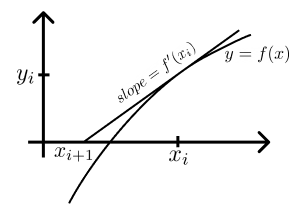
\includegraphics[width=0.45\linewidth]{img/roots_newton}
	\label{fig:rootsnewton}
\end{figure}


Supongamos que ya hemos calculado  $x_i$, calcular  $x_{i+1}$ como sigue. Dibuja la tangente a la gráfica de la función  $f(x)$ en el punto $x = x_i$ , y encuentre el punto de intersección de esta tangente con la $x$-eje. $x_{i+1}$ se iguala a la $x$-coordenada del punto encontrado, y repetimos todo el proceso desde el principio.

No es difícil obtener la siguiente fórmula,

$$ x_{i+1} = x_i - \frac{f(x_i)}{f^\prime(x_i)} $$

Primero calculamos la pendiente $f'(x)$, derivado de $f(x)$, y luego determine la ecuación de la tangente que es,

$$ y - f(x_i) = f'(x_i)(x - x_i) $$

La tangente interseca con el eje x en la coordenada, $y = 0$ y $x = x_{i+1}$,

$$ - f(x_i) = f'(x_i)(x_{i+1} - x_i) $$

Ahora resolviendo la ecuación obtenemos el valor de $x_{i+1}$

Es intuitivamente claro que si la función $f(x)$ es \emph{bueno} (suave), y $x_i$ está lo suficientemente cerca de la raíz, entonces $x_{i+1}$  estará aún más cerca de la raíz deseada.

La tasa de convergencia es cuadrática, lo que, condicionalmente hablando, significa que el número de dígitos exactos en el valor aproximado $x_i$ se duplica con cada iteración.
\section{Implementación}
Usemos el cálculo de la raíz cuadrada como ejemplo del método de Newton. Si sustituimos $f(x) = x^2 - n$ , luego simplificando la expresión obtenemos: 

$$ x_{i+1} = \frac{x_i + \frac{n}{x_i}}{2} $$ 

La primera variante típica del problema es cuando un número racional $n$ se da, y su raíz debe calcularse con cierta precisión $eps$ :

\subsection{C++}
\begin{lstlisting}[language=C++]
double sqrt_newton(double n) {
   const double eps = 1E-15;
   double x = 1;
   for (;;) {
      double nx = (x + n / x) / 2;
      if (abs(x - nx) < eps) break;
      x = nx;
   }
   return x;
}
\end{lstlisting}

\subsection{Java}
\begin{lstlisting}[language=Java]
public static double sqrt_newton(double n) {
   final double eps = 1E-15;
   double x = 1;
   for (;;) {
	double nx = (x + n / x) / 2;
		if (Math.abs(x - nx) < eps) break;
		x = nx;
	}
	return x;
}
\end{lstlisting}

Otra variante común del problema es cuando necesitamos calcular la raíz entera (para el dado $n$  encontrar el más grande $x$ tal que  $x^2 \le n$ ). Aquí es
necesario cambiar ligeramente la condición de terminación del algoritmo, ya que puede suceder que $x$ comenzará a \emph{saltar} cerca de la respuesta. Por lo tanto, agregamos una condición de que si el valor $x$ ha disminuido en el paso anterior e intenta aumentar en el paso actual, entonces se debe
detener el algoritmo.

\subsection{C++}
\begin{lstlisting}[language=C++]
int isqrt_newton(int n) {
   int x = 1;
   bool decreased = false;
   for (;;) {
      int nx = (x + n / x) >> 1;
      if (x == nx || nx > x && decreased) break;
      decreased = nx < x;
      x = nx;
   }
   return x;
}
\end{lstlisting}


\subsection{Java}
\begin{lstlisting}[language=Java]
public static int isqrt_newton(int n) {
   int x = 1;
   boolean decreased = false;
   for (;;) {
      int nx = (x + n / x) >> 1;
      if (x == nx || nx > x && decreased) break;
      decreased = nx < x;
      x = nx;
   }
   return x;
}
\end{lstlisting}

Finalmente, nos dan la tercera variante, para el caso de la aritmética de \emph{bignum}. Desde el número $n$ puede ser lo suficientemente grande, tiene sentido prestar atención a la aproximación inicial. Evidentemente, cuanto más cerca esté de la raíz, más rápido se conseguirá el resultado. Es bastante simple y efectivo tomar la aproximación inicial como el número $2^{\textrm{bits}/2}$ , dónde $\textrm{bits}$ es el número de bits en el número $n$ . Aquí está el código Java que
demuestra esta variante:

\subsection{Java}
\begin{lstlisting}[language=Java]
public static BigInteger isqrtNewton(BigInteger n) {
   BigInteger a = BigInteger.ONE.shiftLeft(n.bitLength() / 2);
   boolean p_dec = false;
   for (;;) {
      BigInteger b = n.divide(a).add(a).shiftRight(1);
      if (a.compareTo(b) == 0 || a.compareTo(b) < 0 && p_dec) break;
      p_dec = a.compareTo(b) > 0;
      a = b;
   }
   return a;
}
\end{lstlisting}
\section{Aplicaciones}
El método de Newton es un método numérico utilizado para encontrar raíces de una función mediante aproximaciones sucesivas. Este método es ampliamente utilizado en diversas áreas de las matemáticas, la ingeniería y la ciencia debido a su eficiencia y rapidez. Algunas aplicaciones del método de Newton para encontrar raíces son:

\begin{enumerate}
\item \textbf{Optimización:} El método de Newton se utiliza en problemas de optimización para encontrar los puntos críticos de una función, es decir, los puntos donde la derivada es igual a cero. Estos puntos pueden corresponder a máximos o mínimos locales de la función.

\item \textbf{Resolución de ecuaciones no lineales:} El método de Newton es útil para resolver ecuaciones no lineales que no tienen solución analítica. Al aplicar el método de Newton, se pueden encontrar las raíces de la ecuación con una buena aproximación.

\item \textbf{Modelado matemático:} En el modelado matemático de fenómenos físicos o biológicos, a menudo se requiere encontrar las raíces de ecuaciones que describen el comportamiento del sistema. El método de Newton es útil para encontrar estas raíces de manera eficiente.

\item \textbf{Análisis numérico:} En el campo del análisis numérico, el método de Newton es una herramienta importante para resolver problemas que involucran funciones no lineales. Se puede utilizar para calcular raíces con alta precisión y rapidez.

\item \textbf{Ingeniería y ciencias aplicadas:} En disciplinas como la ingeniería, la física, la economía y la biología, el método de Newton se utiliza para resolver problemas prácticos que involucran funciones no lineales. Por ejemplo, en ingeniería eléctrica se puede utilizar para analizar circuitos no lineales.
\end{enumerate}

En resumen, el método de Newton es una herramienta poderosa y versátil que se aplica en una amplia variedad de campos para encontrar raíces de funciones de manera eficiente y precisa.
\section{Complejidad}
Por ejemplo, este código se ejecuta en $60$ milisegundos para $n = 10^{1000}$ , y si eliminamos la selección mejorada de la aproximación inicial (empezando simplemente con $1$ ), entonces se ejecutará en aproximadamente $120$ milisegundos.
\section{Ejercicios}
A continuación una lista de ejercicios que se puede resolver aplicando el método abordado en esta guía:

\begin{enumerate}
	\item \href{https://uva.onlinejudge.org/index.php?option=com_onlinejudge&Itemid=8&category=16&page=show_problem&problem=1369}{UVA 10428 - The Roots}
\end{enumerate}
%\section{Anexos}
%\input{tex_files/anexos_successions.tex}


\end{document}